\section{Антенные решётки с равномерным распределением амплитуд и межэлементных расстояний}\label{chap:equally-spaced-arrays}

Основополагающие принципы фазированных антенных решёток были заложены ещё в 1905 году Карлом Фердинандом Брауном,
который получил Нобелевскую премию по физике за разработку методов управления направленностью антенн
с помощью фазового сдвига. Однако широкое применение и разработка таких антенн начались только в середине 20-го века.
Технология начала активно развиваться в 1950-1960х годах в рамках военных и космических программ.
Первые практические применения антенных решёток были связаны с радиолокационными системами для отслеживания
воздушных и космических объектов. 

Классические ФАР представляют собой массив антенных элементов с одинаковыми характеристиками и синфазной запиткой,
расположенными равномерно в линии или на плоскости. Принцип работы ФАР заключается в управлении фазами волн
в антенных элементах таким образом, чтобы через синфазное сложение этих волн с/в определённом направлении достигалось
усиление сигнала, тогда как в других -- ослабление.

На Рисунке~\ref{fig:equally-spaced-distribution} 
показано расположение элементов линейной антенной решётке
и полученные диаграммы направленности в нескольких направлениях

\begin{figure}[!ht]
	\centering
	\begin{subfigure}[b]{0.8\textwidth}
		\centering
		
\includegraphics[width=\textwidth]{equally-spaced-distribution.png}
		\caption{}%
		\label{fig:equally-spaced-distribution-pos}
	\end{subfigure}
	\begin{subfigure}[b]{0.55\textwidth}
		\centering
		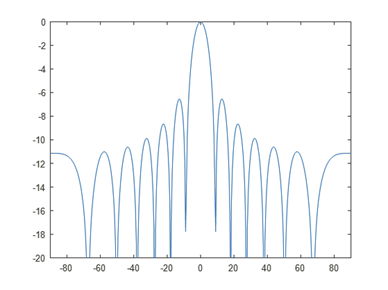
\includegraphics[width=\textwidth]{equally-spaced-distribution-beam-pattern0.png}
		\caption{}%
		\label{fig:equally-spaced-distribution-beam-pattern0}
	\end{subfigure}
	\hfill
	\begin{subfigure}[b]{0.49\textwidth}
		\centering
		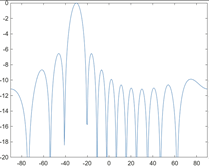
\includegraphics[width=\textwidth]{equally-spaced-distribution-beam-pattern-30.png}
		\caption{}%
		\label{fig:equally-spaced-distribution-beam-pattern-30}
	\end{subfigure}
	\begin{subfigure}[b]{0.49\textwidth}
		\centering
		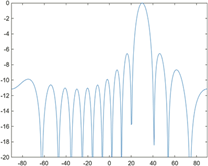
\includegraphics[width=\textwidth]{equally-spaced-distribution-beam-pattern30.png}
		\caption{}%
		\label{fig:equally-spaced-distribution-beam-pattern30}
	\end{subfigure}
	\caption{%
	(а) Расположение элементов 
	ДН при направленности на 
	(б) 0 
	(в) -30 и 
	(г) +30 градусов
	}%
	\label{fig:equally-spaced-distribution}
\end{figure}

Такие антенные решётки применяются и в современных приложениях ввиду простоты их разработки, однако имеют
несколько недостатков: высокий уровень боковых лепестков
(на Рисунке~\ref{fig:equally-spaced-distribution-beam-pattern0}
видно, что уровень второго лепестка составляет порядка -7 дб от основного), увеличение стоимости ввиду
большого количества  элементов, которое требуется для поддержания требуемой ширины основного лепестка при
расстоянии между элементами $d \leq \lambda/2$, либо появление 
дифракционных лепестков (ложных целей) при увеличении межэлементного расстояния,
которое можно увидеть на Рисунке~\ref{fig:equally-spaced-distribution-granting-lobes}

\begin{figure}[ht]
	\centering
	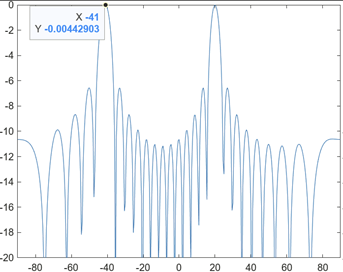
\includegraphics[width=0.8\textwidth,keepaspectratio]{equally-spaced-distribution-granting-lobes.png}
	\caption{ДН при межэлементном расстоянии $d > \lambda/2$, 
	направленность на~20~градусов,
	дифракционный лепесток~на~-41~градус}%
	\label{fig:equally-spaced-distribution-granting-lobes}
\end{figure}

Такие решетки могут применяться в системах, где отсутствие множественной направленности менее критично чем
больший размер/вес итогового устройства, например в системах межспутниковой связи. Кроме того важную роль
играет простота разработки и наладки таких ФАР. 

В системах же, где эти параметры являются критичными, а также в тех случаях когда есть возможность применять
более сложные структуры, применяются решётки, разработанные с помощью методов, которые описаны в следующих
главах.
